% !TEX program = lualatex
\documentclass[11pt]{article}

% -------- LuaLaTeX : polices et langue --------
\usepackage{fontspec}
\setmainfont{Latin Modern Roman}
\setsansfont{Tex Gyre Heros}
%\renewcommand{\familydefault}{\sfdefault} % force le sans serif par défaut
\usepackage{polyglossia}
\setdefaultlanguage{french}

% -------- Mise en page --------
\usepackage[a4paper,margin=1cm]{geometry}
\usepackage{multicol}
\usepackage{fancyhdr}
\pagestyle{empty}
\usepackage[most]{tcolorbox}

% -------- Mathématiques --------
\usepackage{amsmath,amssymb,mathtools}
% \usepackage{siunitx}
% \sisetup{locale=FR}

\usepackage{enumitem}
\setlist[itemize]{left=0pt}
\setlist[enumerate]{left=0pt, label=\textbf{\arabic*}.}

\usepackage{ProfCollege}
\usepackage{ProfMaquette}

%\usepackage{tabularray}
\usepackage{tabularx}

% -------- Divers --------
\newcommand{\ligne}{{\color{gray!60}\hrulefill}}

\setlength{\parindent}{0pt}

\begin{document}



\begin{Maquette}[IE]{
        Numero = 1, Code={}, Date = Jeudi 2 octobre, Theme = Arithmétique / Calcul littéral, Calculatrice = false
    }
    \begin{multicols}{2}

        \begin{exercice}
            \brm{2} Dans le collège, il y a 118 élèves en quatrième. Combien peut-on former d’équipes de baskets de cinq joueurs ? Combien d’élèves restera-t-il ?
        \end{exercice}
        \begin{exercice}
            \begin{enumerate}
                \brm{4}
                \item Écris la liste des huit diviseurs du nombre $30$.
                \item[] \ligne
                \item Donne les deux multiples de $9$ compris entre $100$ et $120$.
                \item[] \ligne
                \item Rappelle la définition d’un nombre \emph{premier}.
                \item[] \ligne
                \item[] \ligne
                \item Écris tous les nombres premiers compris entre $10$ et $30$.
                \item[] \ligne

            \end{enumerate}
        \end{exercice}
        \columnbreak
        \begin{exercice}
            \brm{5}
            \begin{enumerate}
                \item Trouve la décomposition en produit de facteurs premiers des nombres suivants.
                      \begin{multicols}{2}
                          \begin{enumerate}[label=\textbf{\alph*.}]
                              \item $18$
                              \item $30$
                              \item $126$
                              \item $165$
                          \end{enumerate}
                      \end{multicols}
                \item Déduis-en l’écriture irréductible des fractions suivantes.
                      \begin{multicols}{3}
                          \begin{enumerate}[label=\textbf{\alph*.}]
                              \item $\dfrac{30}{18}$
                              \item $\dfrac{18}{126}$
                              \item $\dfrac{30}{165}$
                          \end{enumerate}
                      \end{multicols}
                      \vspace{.5em}
            \end{enumerate}
        \end{exercice}
        
\begin{exercice}
    \brm{5}Recopie et réduis chaque produit.
    \begin{multicols}{3}
        \begin{enumerate}[label=\textbf{\alph*.}]
        \item $6\times x$
        \item $6\times a \times 2$
        \item $y \times 1$
        \item $b \times 3 \times b$
        \item $2x\times 5$
        \item $0 \times t$
        \item $4x \times 10 \times y$
        \item $3a \times 2a$
        \item $e \times 3f \times e$
    \end{enumerate}
    \end{multicols}
\end{exercice}

    \end{multicols}
    \begin{exercice}
        \brm{4}
        \begin{multicols}{2}
            \begin{center}
                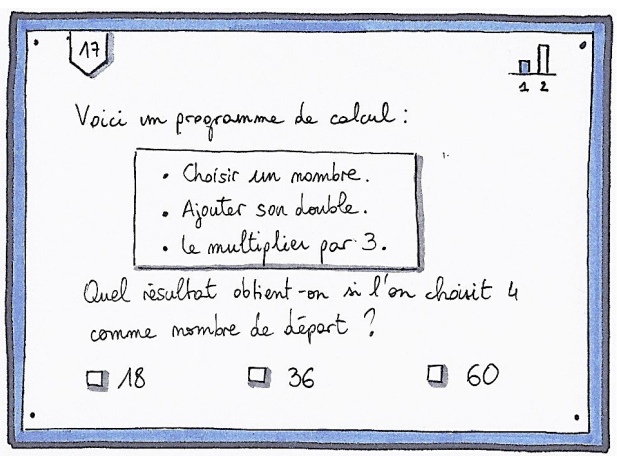
\includegraphics[width=.9\linewidth]{Images/image1.png}

                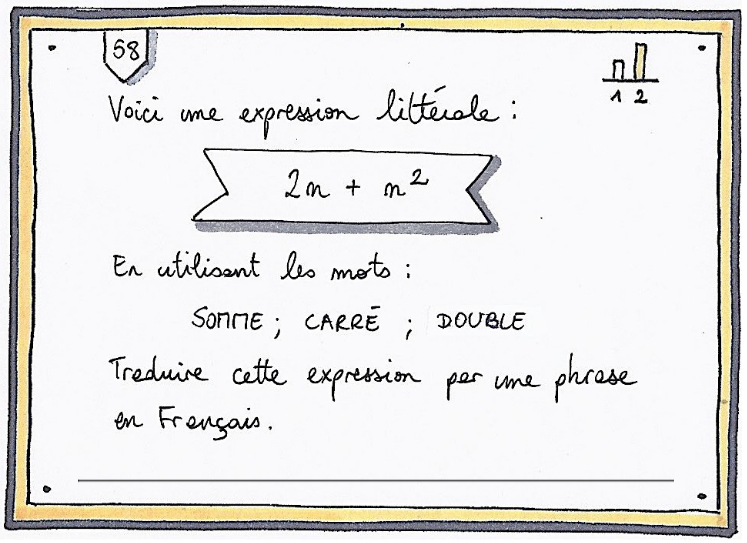
\includegraphics[width=.9\linewidth]{Images/image5.png}

                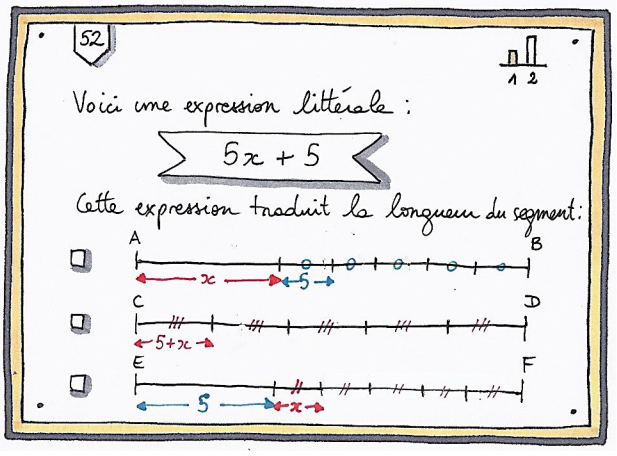
\includegraphics[width=.9\linewidth]{Images/image3.png}

                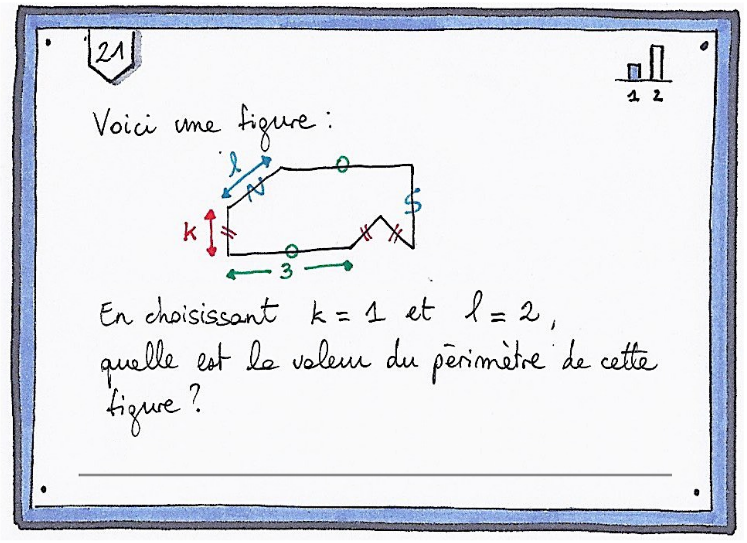
\includegraphics[width=.9\linewidth]{Images/image4.png}
            \end{center}
        \end{multicols}
    \end{exercice}

\end{Maquette}


\end{document}